% answers.tex —— 1977 年·陕西卷 · 参考答案与详细解析片段
% 由 tools/generate_projects.py 依来源总账自 1977/1977_数学真题_陕西_试题.md + 1977/1977_数学真题_陕西_解析正文.md + 1977/1977_数学真题_陕西_答案要点.md 生成，勿手改（改源 MD 后重跑）


\begin{gktip}
固定源是题面与解答连续出现的《陕西1977年高考数学试题解》。下文逐题对照源解答并重新计算关键结论；第 6 题源卷排印中 q 的字形说明见该题源注，参考题两道不计入正式题量。
\end{gktip}

\begin{answer}
\gksolhead{1}{}

\textbf{题目}：

\Needspace{5\baselineskip}
求值：

\nopagebreak[4]
\[
\left(\frac{1}{300}\right)^{-\frac12}
+10\left(\frac{\sqrt3}{2}\right)^{\frac12}\cdot\left(\frac{27}{4}\right)^{\frac14}
-10(2-\sqrt3)^{-1}.
\]

\Needspace{4\baselineskip}
\textbf{解析}

\nopagebreak[4]
\[
\begin{aligned}
&\left(\frac{1}{300}\right)^{-\frac12}
+10\left(\frac{\sqrt3}{2}\right)^{\frac12}\cdot\left(\frac{27}{4}\right)^{\frac14}
-10(2-\sqrt3)^{-1}\\
&=\sqrt{300}
+\frac{10\sqrt[4]{3}}{\sqrt2}\cdot\frac{\sqrt[4]{3^3}}{\sqrt[4]{2^2}}
-\frac{10}{2-\sqrt3}\\
&=10\sqrt3+15-10(2+\sqrt3)\\
&=-5.
\end{aligned}
\]

其中 $\left(\dfrac{1}{300}\right)^{-\frac12}=\sqrt{300}=10\sqrt3$，$10(2-\sqrt3)^{-1}$ 经分母有理化得 $10(2+\sqrt3)$；中间两项相乘得 $\dfrac{10\cdot3}{2}=15$，与前项的 $10\sqrt3$、后项展开的 $10\sqrt3$ 恰好相消。

\gkanswer{答案：$-5$。}

\end{answer}
\begin{answer}
\gksolhead{2}{}

\textbf{题目}：

求值：$\sin480^\circ\cdot\cos480^\circ\cdot\cos960^\circ\cdot\cos1920^\circ$。

\Needspace{4\baselineskip}
\textbf{解析}

\Needspace{5\baselineskip}
由诱导公式，$\sin480^\circ=\sin120^\circ=\dfrac{\sqrt3}{2}$，$\cos480^\circ=\cos120^\circ=-\dfrac12$，$\cos960^\circ=\cos240^\circ=-\dfrac12$，$\cos1920^\circ=\cos120^\circ=-\dfrac12$，因此

\nopagebreak[4]
\[
\sin480^\circ\cdot\cos480^\circ\cdot\cos960^\circ\cdot\cos1920^\circ
=\frac{\sqrt3}{2}\left(-\frac12\right)^3=-\frac{\sqrt3}{16}.
\]

\gkanswer{答案：$-\dfrac{\sqrt3}{16}$。}

\end{answer}
\begin{answer}
\gksolhead{3}{}

\textbf{题目}：

化简：$|6-a|-|2a+1|+\sqrt{a^2+10a+25}$（$a<-5$）。

\Needspace{4\baselineskip}
\textbf{解析}

\Needspace{5\baselineskip}
由 $a<-5$ 得 $6-a>0$、$2a+1<0$、$a+5<0$，故

\nopagebreak[4]
\[
\begin{aligned}
|6-a|-|2a+1|+\sqrt{a^2+10a+25}
&=(6-a)-\left[-(2a+1)\right]+\sqrt{(a+5)^2}\\
&=(6-a)+(2a+1)-(a+5)\\
&=2.
\end{aligned}
\]

\gkanswer{答案：$2$。}

\end{answer}
\begin{answer}
\gksolhead{4}{}

\textbf{题目}：

解不等式：$\lg(2x+1)>\lg(5-x)$。

\Needspace{4\baselineskip}
\textbf{解析}

\Needspace{5\baselineskip}
对数函数当底大于 $1$ 时递增，且真数须为正，故原不等式等价于不等式组

\nopagebreak[4]
\[
\begin{cases}
2x+1>5-x,\\
2x+1>0,\\
5-x>0.
\end{cases}
\]

\Needspace{5\baselineskip}
即 $x>\dfrac43$、$x>-\dfrac12$ 且 $x<5$，因此

\nopagebreak[4]
\[
\frac43<x<5.
\]

（前两条已蕴含 $2x+1>0$，源卷把三条并列是稳妥写法。）

\gkanswer{答案：$\dfrac43<x<5$。}

\end{answer}
\begin{answer}
\gksolhead{5}{}

\textbf{题目}：

设 $A\text{、}B$ 为锐角，且 $\sin A=\dfrac35$，$\sin B=\dfrac5{13}$，求 $\operatorname{tg}(A-B)$。

\Needspace{4\baselineskip}
\textbf{解析}

\Needspace{5\baselineskip}
$A\text{、}B$ 为锐角，故

\nopagebreak[4]
\[
\begin{aligned}
\cos A&=\sqrt{1-\sin^2A}=\sqrt{1-\left(\frac35\right)^2}=\frac45,\\
\cos B&=\sqrt{1-\sin^2B}=\sqrt{1-\left(\frac5{13}\right)^2}=\frac{12}{13}.
\end{aligned}
\]

\Needspace{5\baselineskip}
用差角公式（源卷以 $\operatorname{tg}$ 表示正切，本文按现行记号写 $\tan$）：

\nopagebreak[4]
\[
\tan(A-B)=\frac{\tan A-\tan B}{1+\tan A\tan B}
=\frac{\dfrac34-\dfrac5{12}}{1+\dfrac34\cdot\dfrac5{12}}
=\frac{16}{63}.
\]

\gkanswer{答案：$\dfrac{16}{63}$。}

\end{answer}
\begin{answer}
\gksolhead{6}{}

\textbf{题目}：

实数 $p\text{、}q$ 应满足怎样的条件，才能使方程 $x^2+px+q=0$ 的两根成为一直角三角形两锐角的正弦？

\Needspace{4\baselineskip}
\textbf{解析}

\Needspace{5\baselineskip}
设方程两根为 $x_1\text{、}x_2$，直角三角形一个锐角为 $\alpha$（$0<\alpha<\dfrac\pi2$）。依题意两根为两锐角的正弦，可取

\nopagebreak[4]
\[
x_1=\sin\alpha,
\qquad
x_2=\sin(90^\circ-\alpha)=\cos\alpha.
\]

\Needspace{5\baselineskip}
由韦达定理，

\nopagebreak[4]
\[
\sin\alpha+\cos\alpha=-p,
\qquad
\sin\alpha\cos\alpha=q.
\]

\Needspace{5\baselineskip}
把前式平方，得 $1+2\sin\alpha\cos\alpha=p^2$，代入即得 $p\text{、}q$ 应满足的关系式

\nopagebreak[4]
\[
1+2q=p^2.
\]

\Needspace{5\baselineskip}
再定范围：由 $0<\alpha<\dfrac\pi2$，

\nopagebreak[4]
\[
\sin\alpha+\cos\alpha=\sqrt2\sin\left(\alpha+\frac\pi4\right)\in\left(1,\sqrt2\right],
\]

故 $p=-(\sin\alpha+\cos\alpha)\in[-\sqrt2,-1)$；又 $\sin\alpha\cos\alpha=\dfrac12\sin2\alpha\in\left(0,\dfrac12\right]$。反之，满足这三条的 $p\text{、}q$ 确有相应的 $\alpha$：取 $s=-p\in(1,\sqrt2]$，由 $\sin\alpha+\cos\alpha=s$ 可定出锐角 $\alpha$，此时 $\sin\alpha\cos\alpha=\dfrac{s^2-1}{2}=\dfrac{p^2-1}{2}=q$ 自动成立。所以条件既是必要的也是充分的，$p\text{、}q$ 应满足 $1+2q=p^2$，且 $-\sqrt2\leqslant p<-1$，$0<q\leqslant\dfrac12$。

\begin{gktip}
\textbf{源注}：源卷为打字机排印，同一变量 $q$ 在公式中多处印作形近的“g”字样（如方程印作 $x^2+px+g=0$、关系式一行印作“p、g应满足的关系式”）；按题干“实数 $p\text{、}q$”统一转录为 $q$。
\end{gktip}

\gkanswer{答案：$p\text{、}q$ 应满足 $1+2q=p^2$，且 $-\sqrt2\leqslant p<-1$，$0<q\leqslant\dfrac12$。}

\end{answer}
\begin{answer}
\gksolhead{7}{}

\textbf{题目}：

以任意一点到已知三角形三个顶点连线的中点为顶点作三角形。所作三角形的面积是已知三角形的几倍？

\begin{gktip}
原源 PDF 第 3 页解答处附有点 $P$ 与 $\triangle ABC$ 及中点三角形 $A'B'C'$ 的示意图；LaTeX 版按源图重绘。
\end{gktip}
\nopagebreak[4]
\begin{center}% 1977 年陕西卷第七题：P 为 △ABC 外一点，A′、B′、C′ 分别为 PA、PB、PC 的中点，
% 虚线为中点三角形 A′B′C′（按源卷第 3 页布局：P 左上、A 右上、B 左下、C 右下，C 带实心点）
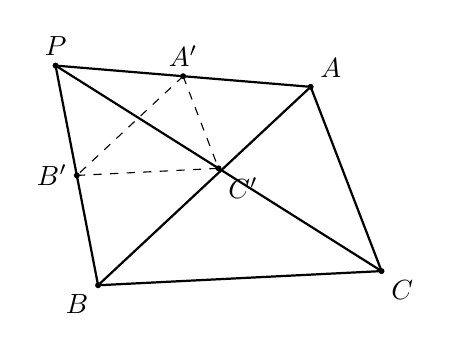
\begin{tikzpicture}[scale=0.9]
  \coordinate (P)  at (0,3.1);
  \coordinate (A)  at (3.6,2.8);
  \coordinate (B)  at (0.6,0);
  \coordinate (C)  at (4.6,0.2);
  \coordinate (Ap) at (1.8,2.95);
  \coordinate (Bp) at (0.3,1.55);
  \coordinate (Cp) at (2.3,1.65);
  \draw[thick] (P)--(A);
  \draw[thick] (P)--(B);
  \draw[thick] (P)--(C);
  \draw[thick] (A)--(B);
  \draw[thick] (B)--(C);
  \draw[thick] (A)--(C);
  \draw[dashed] (Ap)--(Bp);
  \draw[dashed] (Bp)--(Cp);
  \draw[dashed] (Ap)--(Cp);
  \fill (P)  circle (1.2pt) node[above] {$P$};
  \fill (A)  circle (1.2pt) node[above right] {$A$};
  \fill (B)  circle (1.2pt) node[below left] {$B$};
  \fill (C)  circle (1.2pt) node[below right] {$C$};
  \fill (Ap) circle (1.2pt) node[above] {$A'$};
  \fill (Bp) circle (1.2pt) node[left] {$B'$};
  \fill (Cp) circle (1.2pt) node[below right] {$C'$};
\end{tikzpicture}
\end{center}
\nopagebreak[4]
\Needspace{4\baselineskip}
\textbf{解析}
\nopagebreak[4]
\begin{center}% 1977 年陕西卷第七题：P 为 △ABC 外一点，A′、B′、C′ 分别为 PA、PB、PC 的中点，
% 虚线为中点三角形 A′B′C′（按源卷第 3 页布局：P 左上、A 右上、B 左下、C 右下，C 带实心点）
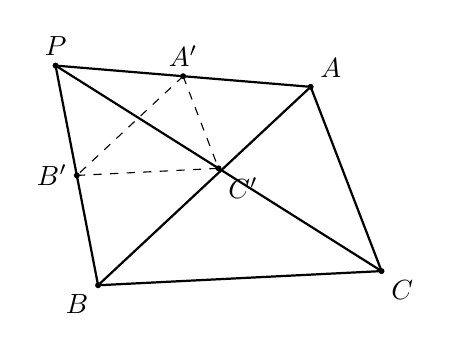
\begin{tikzpicture}[scale=0.9]
  \coordinate (P)  at (0,3.1);
  \coordinate (A)  at (3.6,2.8);
  \coordinate (B)  at (0.6,0);
  \coordinate (C)  at (4.6,0.2);
  \coordinate (Ap) at (1.8,2.95);
  \coordinate (Bp) at (0.3,1.55);
  \coordinate (Cp) at (2.3,1.65);
  \draw[thick] (P)--(A);
  \draw[thick] (P)--(B);
  \draw[thick] (P)--(C);
  \draw[thick] (A)--(B);
  \draw[thick] (B)--(C);
  \draw[thick] (A)--(C);
  \draw[dashed] (Ap)--(Bp);
  \draw[dashed] (Bp)--(Cp);
  \draw[dashed] (Ap)--(Cp);
  \fill (P)  circle (1.2pt) node[above] {$P$};
  \fill (A)  circle (1.2pt) node[above right] {$A$};
  \fill (B)  circle (1.2pt) node[below left] {$B$};
  \fill (C)  circle (1.2pt) node[below right] {$C$};
  \fill (Ap) circle (1.2pt) node[above] {$A'$};
  \fill (Bp) circle (1.2pt) node[left] {$B'$};
  \fill (Cp) circle (1.2pt) node[below right] {$C'$};
\end{tikzpicture}
\end{center}
\nopagebreak[4]
\Needspace{5\baselineskip}
设 $P$ 为 $\triangle ABC$ 外任一点，$A'\text{、}B'\text{、}C'$ 分别是 $PA\text{、}PB\text{、}PC$ 的中点。由三角形中位线的性质，

\nopagebreak[4]
\[
\frac{A'B'}{AB}=\frac{B'C'}{BC}=\frac{A'C'}{AC}=\frac12,
\]

\Needspace{5\baselineskip}
所以 $\triangle A'B'C'\sim\triangle ABC$。两个相似三角形面积之比等于对应边比的平方：

\nopagebreak[4]
\[
\frac{S_{\triangle A'B'C'}}{S_{\triangle ABC}}
=\left(\frac{A'B'}{AB}\right)^2
=\left(\frac12\right)^2
=\frac14,
\qquad
S_{\triangle A'B'C'}=\frac14S_{\triangle ABC}.
\]

即所作三角形的面积是原三角形面积的 $\dfrac14$。

位似观点可统一各种位置：以 $P$ 为位似中心、系数 $\dfrac12$ 的位似把 $A\text{、}B\text{、}C$ 分别映到 $A'\text{、}B'\text{、}C'$，故对 $P$ 在 $\triangle ABC$ 内或边上的情形，面积比同样为 $\dfrac14$，与源卷“若P为已知△ABC内或边上任意一点，也有同样结果，详略”的注记一致。

\gkanswer{答案：所作三角形的面积是已知三角形的 $\dfrac14$。}

\end{answer}
\begin{answer}
\gksolhead{8}{}

\textbf{题目}：

求过椭圆 $\dfrac{x^2}{13^2}+\dfrac{y^2}{12^2}=1$ 的右侧的焦点，且与圆 $x^2+y^2=3^2$ 相切的直线方程。

\Needspace{4\baselineskip}
\textbf{解析}

由半长轴 $a=13$、半短轴 $b=12$ 得 $c=\sqrt{a^2-b^2}=\sqrt{13^2-12^2}=5$，故椭圆右侧焦点为 $(5,0)$。

\Needspace{5\baselineskip}
设切点为 $(x_1,y_1)$，则圆 $x^2+y^2=9$ 在该点的切线方程为

\nopagebreak[4]
\[
x_1x+y_1y=9.
\]

\Needspace{5\baselineskip}
因切线过焦点 $(5,0)$，得 $5x_1=9$；又切点在圆上，得 $x_1^2+y_1^2=9$。联立解得

\nopagebreak[4]
\[
x_1=\frac95,
\qquad
y_1=\pm\frac{12}5.
\]

\Needspace{5\baselineskip}
代入切线方程：

\nopagebreak[4]
\[
\frac95x\pm\frac{12}5y=9
\quad\Longleftrightarrow\quad
9x\pm12y=45
\quad\Longleftrightarrow\quad
3x\pm4y-15=0.
\]

所求直线为 $3x+4y-15=0$ 和 $3x-4y-15=0$。

\gkanswer{答案：$3x+4y-15=0$ 和 $3x-4y-15=0$。}

\end{answer}
\begin{answer}
\gksolhead{9}{}

\textbf{题目}：

三角形的一内角为 $30^\circ$，它的一邻边长为 $4$，对边长为 $\dfrac52$，求另一边长。

\Needspace{4\baselineskip}
\textbf{解析}

\Needspace{5\baselineskip}
设另一边长为 $x$，由余弦定理（$30^\circ$ 角的邻边为 $4$、对边为 $\dfrac52$），

\nopagebreak[4]
\[
\left(\frac52\right)^2=x^2+4^2-2\cdot x\cdot4\cos30^\circ,
\]

\Needspace{5\baselineskip}
即

\nopagebreak[4]
\[
4x^2-16\sqrt3\,x+39=0.
\]

\Needspace{5\baselineskip}
解得

\nopagebreak[4]
\[
x=\frac{16\sqrt3\pm\sqrt{(16\sqrt3)^2-4\cdot4\cdot39}}{8}
=\frac{16\sqrt3\pm12}{8}
=\frac{4\sqrt3\pm3}{2}.
\]

两根均为正且满足三角形不等式，所以三角形另一边长为 $\dfrac{4\sqrt3+3}{2}$ 或 $\dfrac{4\sqrt3-3}{2}$。

\gkanswer{答案：$\dfrac{4\sqrt3+3}{2}$ 或 $\dfrac{4\sqrt3-3}{2}$。}

\end{answer}
\begin{answer}
\gksolhead{10}{}

\textbf{题目}：

在一块边长为 $a$ 的正方形上，切着两边截去了一个半径为 $r$ 的圆料（$r\leqslant\dfrac{(2-\sqrt2)a}{4}$），如果象图 1 那样截出一个正方形的料，它的面积为多大？如果象图 2 那样截出的一个正方形的料，它的面积为多大？这二种截法截下的正方形的料的面积哪个较大？

\begin{gktip}
原源 PDF 第 5 页解答处附有图 1、图 2 两幅示意图；LaTeX 版按源图重绘。
\end{gktip}
\nopagebreak[4]
\begin{center}% 1977 年陕西卷第十题图 1：正方形 ABCD 的角 B 处切着两边截去半径为 r 的圆料，
% 截出的正方形 A′B′C′D 与原正方形共角 D，顶点 B′ 落在对角线 BD 与圆的交点处（按源卷第 5 页布局）
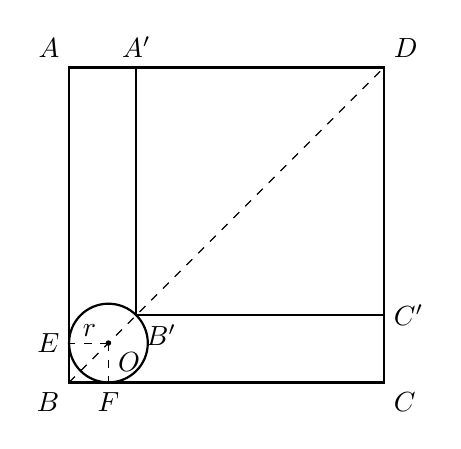
\begin{tikzpicture}[scale=1.0]
  \draw[thick] (0,0)--(4,0)--(4,4)--(0,4)--cycle;
  \draw[thick] (0.8536,4)--(0.8536,0.8536);
  \draw[thick] (0.8536,0.8536)--(4,0.8536);
  \draw[thick] (0.5,0.5) circle (0.5);
  \draw[dashed] (0,0)--(4,4);
  \draw[dashed] (0.5,0.5)--(0,0.5);
  \draw[dashed] (0.5,0.5)--(0.5,0);
  \fill (0.5,0.5) circle (1pt) node[below right] {$O$};
  \node at (0.26,0.66) {$r$};
  \node[left]  at (0,0.5)   {$E$};
  \node[below] at (0.5,0)   {$F$};
  \node[above left]  at (0,4)      {$A$};
  \node[above]       at (0.8536,4) {$A'$};
  \node[above right] at (4,4)      {$D$};
  \node[right]  at (4,0.8536) {$C'$};
  \node[below right] at (4,0)      {$C$};
  \node[below left]  at (0,0)      {$B$};
  \node[below right] at (0.8536,0.8536) {$B'$};
\end{tikzpicture}
\end{center}
\nopagebreak[4]
\nopagebreak[4]
\begin{center}% 1977 年陕西卷第十题图 2：圆与两边 AB、BC 相切于 E、F，且与内接正方形 A′B′C′D′ 的边 A′B′ 相切于 G
% （顶点标注按解答正文用 D′；源图该点印作 D，撇号系描图脱落）
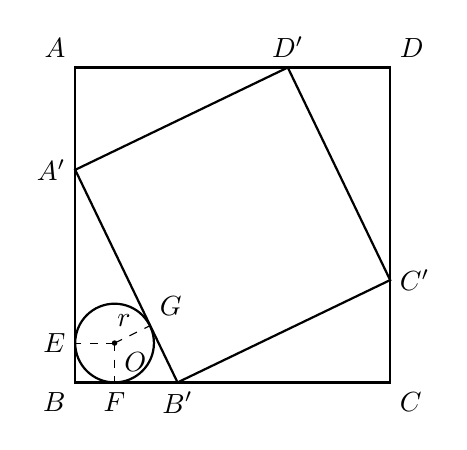
\begin{tikzpicture}[scale=1.0]
  \draw[thick] (0,0)--(4,0)--(4,4)--(0,4)--cycle;
  \draw[thick] (0,2.7)--(1.3,0)--(4,1.3)--(2.7,4)--cycle;
  \draw[thick] (0.5,0.5) circle (0.5);
  \draw[dashed] (0.5,0.5)--(0,0.5);
  \draw[dashed] (0.5,0.5)--(0.5,0);
  \draw[dashed] (0.5,0.5)--(0.95,0.72);
  \fill (0.5,0.5) circle (1pt) node[below right] {$O$};
  \node at (0.62,0.78) {$r$};
  \node[above right] at (0.95,0.72) {$G$};
  \node[left]  at (0,0.5) {$E$};
  \node[below] at (0.5,0) {$F$};
  \node[above left]  at (0,4)    {$A$};
  \node[left]        at (0,2.7)  {$A'$};
  \node[above]       at (2.7,4)  {$D'$};
  \node[above right] at (4,4)    {$D$};
  \node[right]       at (4,1.3)  {$C'$};
  \node[below left]  at (0,0)    {$B$};
  \node[below]       at (1.3,0)  {$B'$};
  \node[below right] at (4,0)    {$C$};
\end{tikzpicture}
\end{center}
\nopagebreak[4]
\textbf{参考题 1．} 在一个椭圆的所有内接矩形中，怎样的矩形面积最大？

\begin{gktip}
原源 PDF 第 6 页解答处附有椭圆与内接矩形的示意图；LaTeX 版按源图重绘。
\end{gktip}
\nopagebreak[4]
\begin{center}% 1977 年陕西卷参考题一：椭圆 x^2/a^2 + y^2/b^2 = 1 的内接矩形 ABCD，
% 长 AD=2x、宽 CD 为纵弦，x 轴标 ±a、y 轴标 ±b（按源卷第 6 页布局）
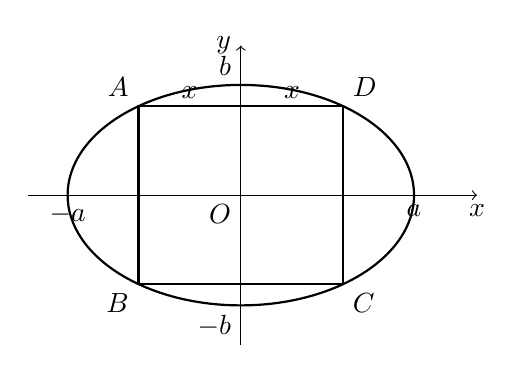
\begin{tikzpicture}[scale=1.0]
  \draw[->] (-2.7,0)--(3.0,0) node[below] {$x$};
  \draw[->] (0,-1.9)--(0,1.9) node[left] {$y$};
  \draw[thick] (0,0) ellipse (2.2 and 1.4);
  \draw[thick] (-1.3,-1.13) rectangle (1.3,1.13);
  \node[above left]  at (-1.3,1.13)  {$A$};
  \node[above right] at (1.3,1.13)   {$D$};
  \node[below left]  at (-1.3,-1.13) {$B$};
  \node[below right] at (1.3,-1.13)  {$C$};
  \node at (-0.65,1.3) {$x$};
  \node at (0.65,1.3)  {$x$};
  \node[below left]  at (0,0)     {$O$};
  \node[below]       at (-2.2,0)  {$-a$};
  \node[below]       at (2.2,0)   {$a$};
  \node[above left]  at (0,1.4)   {$b$};
  \node[below left]  at (0,-1.4)  {$-b$};
\end{tikzpicture}
\end{center}
\nopagebreak[4]
\Needspace{5\baselineskip}
\textbf{参考题 2．} 试解

\nopagebreak[4]
\[
\frac{dy}{dx}-2xy=2x^3,
\qquad
y\Big|_{x=0}=1.
\]

\Needspace{4\baselineskip}
\textbf{解析}
\nopagebreak[4]
\begin{center}% 1977 年陕西卷第十题图 1：正方形 ABCD 的角 B 处切着两边截去半径为 r 的圆料，
% 截出的正方形 A′B′C′D 与原正方形共角 D，顶点 B′ 落在对角线 BD 与圆的交点处（按源卷第 5 页布局）
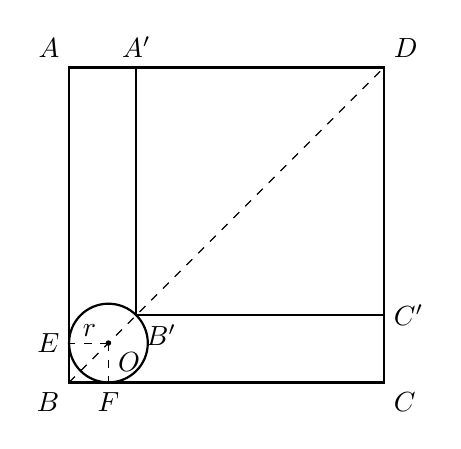
\begin{tikzpicture}[scale=1.0]
  \draw[thick] (0,0)--(4,0)--(4,4)--(0,4)--cycle;
  \draw[thick] (0.8536,4)--(0.8536,0.8536);
  \draw[thick] (0.8536,0.8536)--(4,0.8536);
  \draw[thick] (0.5,0.5) circle (0.5);
  \draw[dashed] (0,0)--(4,4);
  \draw[dashed] (0.5,0.5)--(0,0.5);
  \draw[dashed] (0.5,0.5)--(0.5,0);
  \fill (0.5,0.5) circle (1pt) node[below right] {$O$};
  \node at (0.26,0.66) {$r$};
  \node[left]  at (0,0.5)   {$E$};
  \node[below] at (0.5,0)   {$F$};
  \node[above left]  at (0,4)      {$A$};
  \node[above]       at (0.8536,4) {$A'$};
  \node[above right] at (4,4)      {$D$};
  \node[right]  at (4,0.8536) {$C'$};
  \node[below right] at (4,0)      {$C$};
  \node[below left]  at (0,0)      {$B$};
  \node[below right] at (0.8536,0.8536) {$B'$};
\end{tikzpicture}
\end{center}
\nopagebreak[4]
\nopagebreak[4]
\begin{center}% 1977 年陕西卷第十题图 2：圆与两边 AB、BC 相切于 E、F，且与内接正方形 A′B′C′D′ 的边 A′B′ 相切于 G
% （顶点标注按解答正文用 D′；源图该点印作 D，撇号系描图脱落）
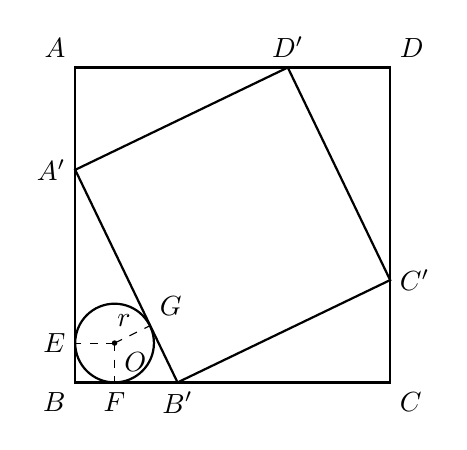
\begin{tikzpicture}[scale=1.0]
  \draw[thick] (0,0)--(4,0)--(4,4)--(0,4)--cycle;
  \draw[thick] (0,2.7)--(1.3,0)--(4,1.3)--(2.7,4)--cycle;
  \draw[thick] (0.5,0.5) circle (0.5);
  \draw[dashed] (0.5,0.5)--(0,0.5);
  \draw[dashed] (0.5,0.5)--(0.5,0);
  \draw[dashed] (0.5,0.5)--(0.95,0.72);
  \fill (0.5,0.5) circle (1pt) node[below right] {$O$};
  \node at (0.62,0.78) {$r$};
  \node[above right] at (0.95,0.72) {$G$};
  \node[left]  at (0,0.5) {$E$};
  \node[below] at (0.5,0) {$F$};
  \node[above left]  at (0,4)    {$A$};
  \node[left]        at (0,2.7)  {$A'$};
  \node[above]       at (2.7,4)  {$D'$};
  \node[above right] at (4,4)    {$D$};
  \node[right]       at (4,1.3)  {$C'$};
  \node[below left]  at (0,0)    {$B$};
  \node[below]       at (1.3,0)  {$B'$};
  \node[below right] at (4,0)    {$C$};
\end{tikzpicture}
\end{center}
\nopagebreak[4]
\Needspace{5\baselineskip}
\textbf{第一种截法（图 1）。} 设 $\odot O$ 与正方形 $ABCD$ 的边 $AB\text{、}BC$ 分别相切于 $E\text{、}F$，则 $OEBF$ 为正方形，圆心 $O$ 在对角线 $BD$ 上，且

\nopagebreak[4]
\[
BD=\sqrt2\,a,
\qquad
OB=\sqrt2\,r.
\]

\Needspace{5\baselineskip}
截出的正方形 $A'B'C'D$ 与原正方形共角 $D$，其顶点 $B'$ 落在对角线 $BD$ 与圆的交点处：

\nopagebreak[4]
\[
B'D=BD-BB'=\sqrt2\,a-(\sqrt2\,r+r).
\]

\Needspace{5\baselineskip}
$B'D$ 是小正方形的对角线，于是

\nopagebreak[4]
\[
\begin{aligned}
S_{A'B'C'D}
&=\frac12\,B'D\cdot B'D\sin90^\circ\\
&=\frac12\left[\sqrt2\,a-(\sqrt2\,r+r)\right]^2\\
&=\left[a-\left(1+\frac{\sqrt2}{2}\right)r\right]^2.
\end{aligned}
\]

小正方形的两边过圆与对角线的交点 $B'$，与圆料只在角点 $B'$ 处相触，不发生重叠。

\Needspace{5\baselineskip}
\textbf{第二种截法（图 2）。} 设 $\odot O$ 与边 $AB\text{、}BC$ 分别相切于 $E\text{、}F$，与内接正方形 $A'B'C'D'$ 的边 $A'B'$ 相切于 $G$。由 $A'B'\perp A'D'$、$AB\perp AD$ 得 $\angle AD'A'=\angle BA'B'$，而 $A'D'=A'B'$，$\angle A=\angle B=90^\circ$，所以

\nopagebreak[4]
\[
\mathrm{Rt}\triangle AD'A'\cong\mathrm{Rt}\triangle A'BB',
\]

\Needspace{5\baselineskip}
从而 $AA'=BB'$。又自 $A'$ 向圆所作的两条切线长相等，$A'G=A'E$；自 $B'$ 亦有 $B'G=B'F$。于是

\nopagebreak[4]
\[
A'G=A'E=AB-AA'-EB=a-(r+FB')-r=a-2r-FB',
\]

\Needspace{5\baselineskip}
而 $B'G=B'F=FB'$，故

\nopagebreak[4]
\[
A'B'=A'G+B'G=a-2r-FB'+FB'=a-2r.
\]

\Needspace{5\baselineskip}
所以

\nopagebreak[4]
\[
S_{A'B'C'D'}=(A'B')^2=(a-2r)^2.
\]

\Needspace{5\baselineskip}
\textbf{比较。} 由 $1+\dfrac{\sqrt2}{2}<2$ 得

\nopagebreak[4]
\[
\left[a-\left(1+\frac{\sqrt2}{2}\right)r\right]^2>(a-2r)^2,
\]

因此第一种截法（如图 1）截下的正方形料的面积较大。

\textbf{参考题 1}

\Needspace{4\baselineskip}
\textbf{解析}
\nopagebreak[4]
\begin{center}% 1977 年陕西卷参考题一：椭圆 x^2/a^2 + y^2/b^2 = 1 的内接矩形 ABCD，
% 长 AD=2x、宽 CD 为纵弦，x 轴标 ±a、y 轴标 ±b（按源卷第 6 页布局）
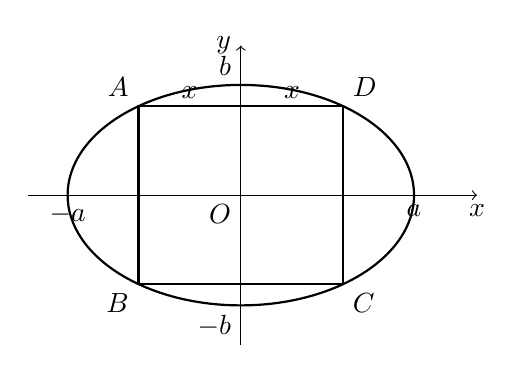
\begin{tikzpicture}[scale=1.0]
  \draw[->] (-2.7,0)--(3.0,0) node[below] {$x$};
  \draw[->] (0,-1.9)--(0,1.9) node[left] {$y$};
  \draw[thick] (0,0) ellipse (2.2 and 1.4);
  \draw[thick] (-1.3,-1.13) rectangle (1.3,1.13);
  \node[above left]  at (-1.3,1.13)  {$A$};
  \node[above right] at (1.3,1.13)   {$D$};
  \node[below left]  at (-1.3,-1.13) {$B$};
  \node[below right] at (1.3,-1.13)  {$C$};
  \node at (-0.65,1.3) {$x$};
  \node at (0.65,1.3)  {$x$};
  \node[below left]  at (0,0)     {$O$};
  \node[below]       at (-2.2,0)  {$-a$};
  \node[below]       at (2.2,0)   {$a$};
  \node[above left]  at (0,1.4)   {$b$};
  \node[below left]  at (0,-1.4)  {$-b$};
\end{tikzpicture}
\end{center}
\nopagebreak[4]
\Needspace{5\baselineskip}
设椭圆的方程为

\nopagebreak[4]
\[
\frac{x^2}{a^2}+\frac{y^2}{b^2}=1.
\]

\Needspace{5\baselineskip}
若内接矩形 $ABCD$ 的长 $AD=2x$（如图，$A\text{、}D$ 在上半椭圆，$B\text{、}C$ 为其关于 $x$ 轴的对称点），则矩形的宽

\nopagebreak[4]
\[
CD=\frac{2b}{a}\sqrt{a^2-x^2}.
\]

\Needspace{5\baselineskip}
这时矩形的面积

\nopagebreak[4]
\[
\begin{aligned}
S(x)
&=\frac{4b}{a}\,x\sqrt{a^2-x^2}
=\frac{4b}{a}\sqrt{x^2\left(a^2-x^2\right)}\\
&\leqslant\frac{4b}{a}\cdot\frac{x^2+\left(a^2-x^2\right)}{2}\\
&=2ab
\qquad\text{（\text{常数}）}.
\end{aligned}
\]

\Needspace{5\baselineskip}
其中不等式中的等号，在 $x^2=a^2-x^2$ 即 $x=\dfrac{\sqrt2}{2}a$ 时成立，此时 $S(x)$ 有最大值 $2ab$。这时

\nopagebreak[4]
\[
AD=2x=\sqrt2\,a,
\qquad
CD=\frac{2b}{a}\sqrt{a^2-\frac{a^2}{2}}=\sqrt2\,b.
\]

答：当内接矩形的长和宽分别是椭圆的半长轴和半短轴的 $\sqrt2$ 倍时，面积最大。

\textbf{参考题 2}

\Needspace{4\baselineskip}
\textbf{解析}

\Needspace{5\baselineskip}
记 $t=x^2$，则 $\dfrac{dy}{dx}=\dfrac{dy}{dt}\cdot\dfrac{dt}{dx}=2x\dfrac{dy}{dt}$，原方程化为

\nopagebreak[4]
\[
2x\frac{dy}{dt}-2xy=2x^3,
\]

\Needspace{5\baselineskip}
消去 $2x$ 即

\nopagebreak[4]
\[
\frac{dy}{dt}-y=t.
\]

\Needspace{5\baselineskip}
相应的齐次方程 $\dfrac{dy}{dt}-y=0$ 的特征根为 $1$，通解为 $y=ce^t$；易验证 $y=-t-1$ 是原方程的一个特解，因此

\nopagebreak[4]
\[
y=ce^t-t-1.
\]

\Needspace{5\baselineskip}
代回原变量 $t=x^2$，得到原方程的通解

\nopagebreak[4]
\[
y=ce^{x^2}-x^2-1.
\]

\Needspace{5\baselineskip}
代入初值条件 $y\Big|_{x=0}=1$，得 $c-1=1$，定出 $c=2$。所以原方程初值问题的解为

\nopagebreak[4]
\[
y=2e^{x^2}-x^2-1.
\]

\gkanswer{答案：图 1 截法截得的正方形面积为 $\left[a-\left(1+\dfrac{\sqrt2}{2}\right)r\right]^2$，图 2 截法截得的正方形面积为 $(a-2r)^2$；第一种截法（图 1）截下的正方形料面积较大。}

\end{answer}